\begin{figure*}[ht]
  \centering
  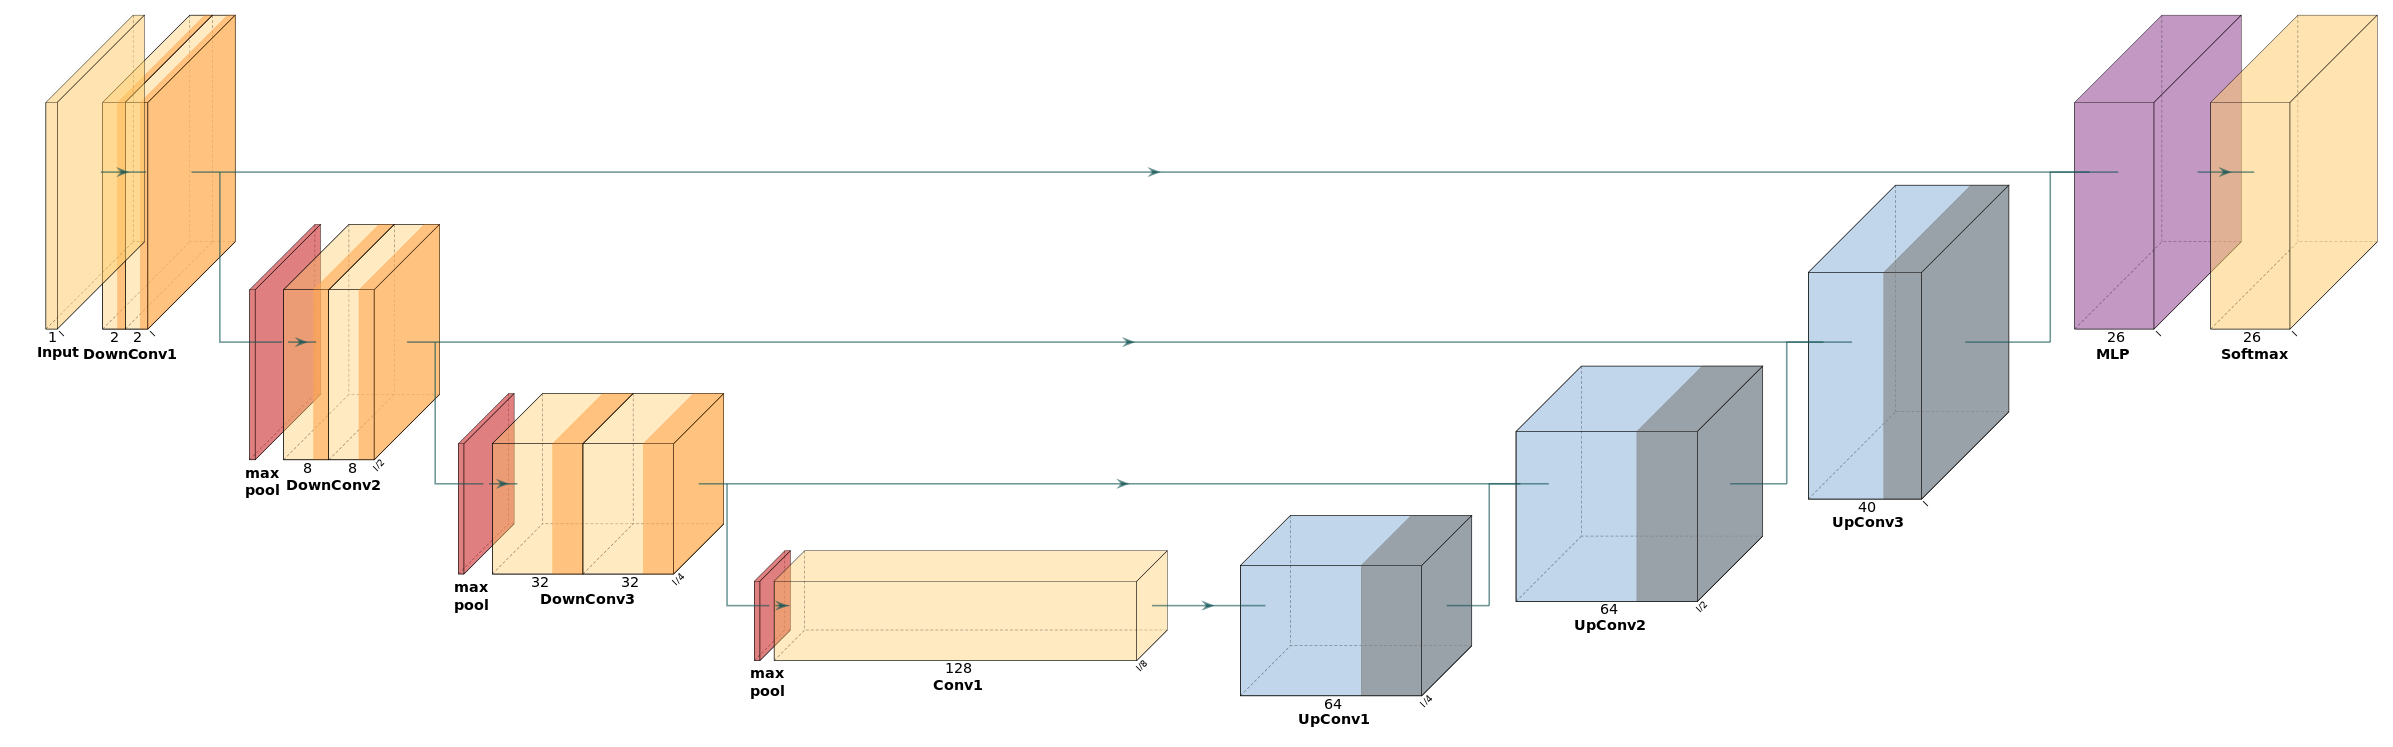
\includegraphics[width=\textwidth]{images/VUE_net_model.png}
  \caption{VUE-net architecture}
  \label{fig:model}
\end{figure*}

Because of the similarity of our task with image encoding, we decided to take inspiration for our model architecture
from many different networks used for image segmentation. Our main inspiration was U-net \cite{Unet}.
This network exploits an autoencorder-like architecture to obtain the segmented image.
In particular, it uses convolution to extract features and maxpooling to downsample the image.
Another U-net element that inspired us is the use of concatenation in order to provide
residual connections between the "down" and "up" convolutions of the image. It must be noted that
the authors of the paper used cropping in order to perform these operations, as the feature dimensions between layers do not exactly match. 
It will be shown later that our architecture does not suffer from this issue since we decided to simplify 
this process by having hidden states of equal size.
Another model architecture we took inspiration from was VoxSegNet \cite{VoxSegNet}. This architecture performs 
sequential extraction of features that are combined toghether, across different levels of extraction, to obtain a prediction. 
This is analogous to the residual but with some additional complexity that won't be
further explained in this paper. 
The specific VoxSegNet element we included in our model architecture is the use of convolutional layers with different dilation rates 
(atrous convolutions) in order to obtain features through kernels with different receptive fields.

Figure \ref{fig:model} illustrates the complete scheme of our model architecture, which is now going to be discussed.
For the down-convolution steps we used a custom \textit{DownConv} layer that consists in two different
convolution layers, one with a dilation rate of 2 and a traditional one, which both double the number of features. 
The output of this layer is the concatenation of the results of the two convolutions.
Between steps, max pooling has been adopted to extract the more relevant features and to compress the representation.
At the "bottom" of the "convolutional ladder" a standard convolution that doubles the number of features has been used.
Then, each one of the up-convolution (also known as transposed convolution) steps is executed by a \textit{UpConv} layer that halves the number of features
and increases the other dimensions, therefore expanding the data representation untill layer \textit{UpConv3} matches the input dimensions.
As shown in the figure, this leads to a features number unbalance towards the ones coming from up-convolutions.
This was purposly done to give more importance to features of the new data representation that is expected to be more 
contiguos with respect to the original one that is affected by sparsity caused by the pointclouds sampling mentioned earlier.
In the end, a multi-layer perceptron (\textit{MLP}), made of two fully connected layers, has been used
to shrink the features dimensions to the number of classes (26) combined with a SoftMax layer that allows
to have the desired probability distribution.
Additionaly, between every subsequent convolutions batch normalization layers and ReLU activation functions were used.
This choice was made to stabilize the outputs of each layer and avoid overfitting. The ReLU in particular was chosen for
its general reliability and simplicity, as no particular properties were required
for the values of the in-between layers.

To obtain more accurate predictions, we created an additional model that exploits the previous
one robustness to input rotations which, as it will be explained later, is embedded at training time.
This network feeds the original model with the four possibile rotated versions of the given sample, 
aligns the received labels and returns their mean values.
